\chapter{Joshua 8}

\begin{figure}
  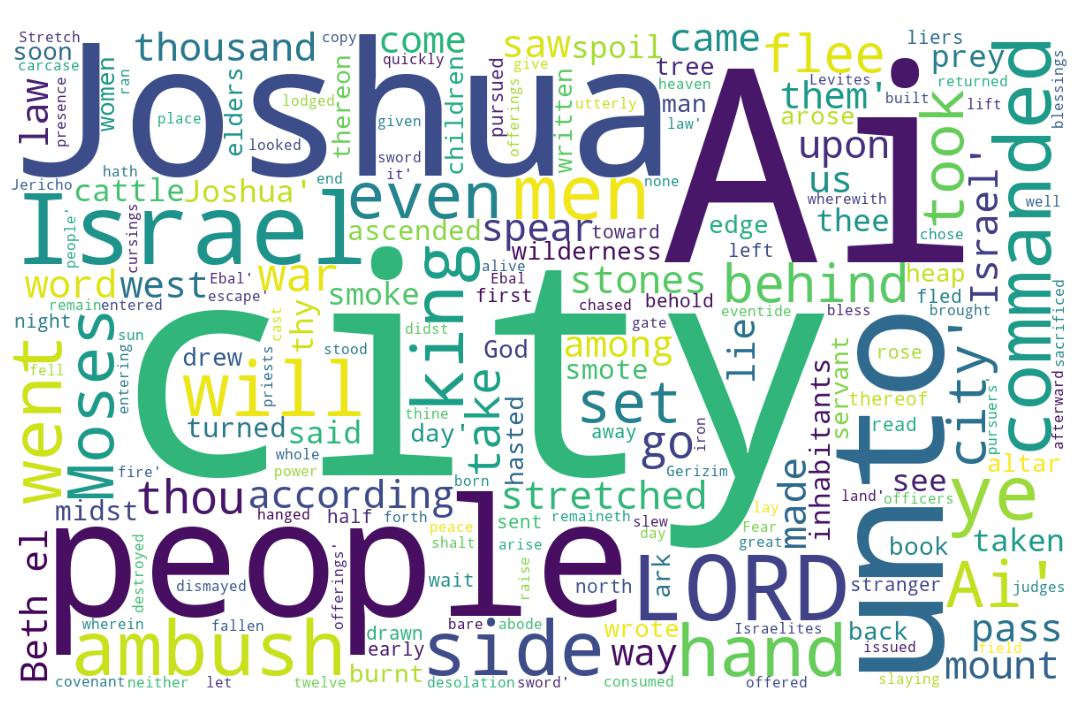
\includegraphics[width=\linewidth]{06OT-Joshua/Joshua8-WordCloud.jpg}
  \caption{Joshua 8 Word Cloud}
  \label{fig:Joshua 8 Word Cloud}
\end{figure}

\marginpar{\scriptsize \centering \fcolorbox{bone}{lime}{\textbf{ACHIN FOR A BRUSIN'}}\\ (Joshua 8)

\begin{compactenum}[I.][8]

	\item A \textbf{Never-Ending Promise} \index[scripture]{Joshua!Jsh 08:01}  (Jsh 8:1) 
	\item \textbf{No Procrastination} \index[scripture]{Joshua!Jsh 08:03}  (Jsh 8:3) 
	\item A \textbf{Nifty Plan} \index[scripture]{Joshua!Jsh 08:07}  (Jsh 8:7) 
	\item An \textbf{Unwise Pursuit} \index[scripture]{Joshua!Jsh 08:16--17}  (Jsh 8:16--17) 
	\item The \textbf{Number who Perished} \index[scripture]{Joshua!Jsh 08:25}  (Jsh 8:25) 
	\item A \textbf{National Presence} \index[scripture]{Joshua!Jsh 08:32}  (Jsh 8:32) 
	\item A \textbf{Notable Publication} \index[scripture]{Joshua!Jsh 08:34}  (Jsh 8:34) 
\end{compactenum}}


\footnote{\textcolor[cmyk]{0.99998,1,0,0}{\hyperlink{TOC}{Return to end of Table of Contents.}}}\textcolor[cmyk]{0.99998,1,0,0}{And the LORD said unto Joshua, Fear not, neither be thou dismayed: take all the \fcolorbox{bone}{bone}{people} of war with thee, and arise, go up to Ai: see, \fcolorbox{bone}{lime}{I have} \fcolorbox{bone}{lime}{blue}{given} into thy hand the king of Ai, and his \fcolorbox{bone}{bone}{people}, and his city, and his land:}
[2] \textcolor[cmyk]{0.99998,1,0,0}{And thou shalt do to Ai and her king as thou didst unto Jericho and her king: only the spoil thereof, and the cattle thereof, shall ye take for a prey unto yourselves: lay thee an ambush for the city behind it.}\\
\\
\P \textcolor[cmyk]{0.99998,1,0,0}{So Joshua arose, and all the \fcolorbox{bone}{bone}{people} of war, to go up against Ai: and Joshua chose out thirty thousand mighty men of valour, and \fcolorbox{bone}{lime}{sent them} \fcolorbox{bone}{lime}{away} by night.}
[4] \textcolor[cmyk]{0.99998,1,0,0}{And he commanded them, saying, Behold, ye shall lie in wa\fcolorbox{bone}{bone}{it} against the city, \emph{even} behind the city: go not very far from the city, but be ye all ready:}
[5] \textcolor[cmyk]{0.99998,1,0,0}{And I, and all the \fcolorbox{bone}{bone}{people} that \emph{are} with me, will approach unto the city: and \fcolorbox{bone}{bone}{it} shall come to pass, when they come out against us, as at the first, that we will flee before them,}
[6] \textcolor[cmyk]{0.99998,1,0,0}{(For they will come out after us) till we have drawn them from the city; for they will say, They flee before us, as at the first: therefore we will flee before them.}
[7] \textcolor[cmyk]{0.99998,1,0,0}{Then ye shall rise up from the ambush, and seize upon the city: for the LORD your \fcolorbox{bone}{lime}{God will deliver} \fcolorbox{bone}{bone}{it} into your hand.}
[8] \textcolor[cmyk]{0.99998,1,0,0}{And \fcolorbox{bone}{bone}{it} shall be, when ye have taken the city, \emph{that} ye shall set the city \fcolorbox{bone}{bone}{on} fire: according to the commandment of the LORD shall ye do. See, I have commanded you.}\\
\\
\P \textcolor[cmyk]{0.99998,1,0,0}{Joshua therefore sent them forth: and they went to lie in ambush, and abode between Beth-el and Ai, \fcolorbox{bone}{bone}{on} the west side of Ai: but Joshua lodged that night among the \fcolorbox{bone}{bone}{people}.}
[10] \textcolor[cmyk]{0.99998,1,0,0}{And Joshua rose up early in the morning, and numbered the \fcolorbox{bone}{bone}{people}, and went up, he and the elders of Israel, before the \fcolorbox{bone}{bone}{people} to Ai.}
[11] \textcolor[cmyk]{0.99998,1,0,0}{And all the \fcolorbox{bone}{bone}{people}, \emph{even} \emph{the} \emph{people} of war that \emph{were} with him, went up, and drew nigh, and came before the city, and pitched \fcolorbox{bone}{bone}{on} the north side of Ai: now \emph{there} \emph{was} a valley between them and Ai.}
[12] \textcolor[cmyk]{0.99998,1,0,0}{And he took about five thousand men, and set them to lie in ambush between Beth-el and Ai, \fcolorbox{bone}{bone}{on} the west side of the city.}
[13] \textcolor[cmyk]{0.99998,1,0,0}{And when they had set the \fcolorbox{bone}{bone}{people}, \emph{even} all the host that \emph{was} \fcolorbox{bone}{bone}{on} the north of the city, and their liers in wa\fcolorbox{bone}{bone}{it} \fcolorbox{bone}{bone}{on} the west of the city, Joshua went that night into the midst of the valley.}\\
\\
\P \textcolor[cmyk]{0.99998,1,0,0}{And \fcolorbox{bone}{bone}{it} came to pass, when the king of Ai saw \emph{it}, that they hasted and rose up early, and the men of the city went out against Israel to battle, he and all his \fcolorbox{bone}{bone}{people}, at a time appointed, before the plain; but he wist not that \emph{there} \emph{were} liers in ambush against him behind the city.}
[15] \textcolor[cmyk]{0.99998,1,0,0}{And Joshua and all Israel made as if they were beaten before them, and fled by the way of the wilderness.}
[16] \textcolor[cmyk]{0.99998,1,0,0}{And all the \fcolorbox{bone}{bone}{people} that \emph{were} in Ai were called together to \fcolorbox{bone}{lime}{pursue} after them: and they pursued after Joshua, and were drawn away from the city.}
[17] \textcolor[cmyk]{0.99998,1,0,0}{And there was not a man left in Ai or Beth-el, that went not out after Israel: and they left the city open, and pursued after Israel.}
[18] \textcolor[cmyk]{0.99998,1,0,0}{And the LORD said unto Joshua, Stretch out the spear that \emph{is} in thy hand toward Ai; for I will give \fcolorbox{bone}{bone}{it} into thine hand. And Joshua stretched out the spear that \emph{he} \emph{had} in his hand toward the city.}
[19] \textcolor[cmyk]{0.99998,1,0,0}{And the ambush arose quickly out of their place, and they ran as soon as he had stretched out his hand: and they entered into the city, and took it, and hasted and set the city \fcolorbox{bone}{bone}{on} fire.}
[20] \textcolor[cmyk]{0.99998,1,0,0}{And when the men of Ai looked behind them, they saw, and, behold, the smoke of the city ascended up to heaven, and they had no power to flee this way or that way: and the \fcolorbox{bone}{bone}{people} that fled to the wilderness turned back upon the pursuers.}
[21] \textcolor[cmyk]{0.99998,1,0,0}{And when Joshua and all Israel saw that the ambush had taken the city, and that the smoke of the city ascended, then they turned again, and slew the men of Ai.}
[22] \textcolor[cmyk]{0.99998,1,0,0}{And the other issued out of the city against them; so they were in the midst of Israel, some \fcolorbox{bone}{bone}{on} this side, and some \fcolorbox{bone}{bone}{on} that side: and they smote them, so that they let none of them remain or escape.}
[23] \textcolor[cmyk]{0.99998,1,0,0}{And the king of Ai they took alive, and brought him to Joshua.}
[24] \textcolor[cmyk]{0.99998,1,0,0}{And \fcolorbox{bone}{bone}{it} came to pass, when Israel had made an end of slaying all the inhabitants of Ai in the field, in the wilderness wherein they chased them, and when they were all fallen \fcolorbox{bone}{bone}{on} the edge of the sword, until they were consumed, that all the Israelites returned unto Ai, and smote \fcolorbox{bone}{bone}{it} with the edge of the sword.}
[25] \textcolor[cmyk]{0.99998,1,0,0}{And \emph{so} \fcolorbox{bone}{bone}{it} was, \emph{that} all that fell that day, both of men and women, \emph{were} \fcolorbox{bone}{lime}{twelve thousand}, \emph{even} all the men of Ai.}
[26] \textcolor[cmyk]{0.99998,1,0,0}{For Joshua drew not his hand back, wherewith he stretched out the spear, until he had utterly destroyed all the inhabitants of Ai.}
[27] \textcolor[cmyk]{0.99998,1,0,0}{Only the cattle and the spoil of that city Israel took for a prey unto themselves, according unto the word of the LORD which he commanded Joshua.}
[28] \textcolor[cmyk]{0.99998,1,0,0}{And Joshua burnt Ai, and made \fcolorbox{bone}{bone}{it} an heap for ever, \emph{even} a desolation unto this day.}
[29] \textcolor[cmyk]{0.99998,1,0,0}{And the king of Ai he hanged \fcolorbox{bone}{bone}{on} a tree until eventide: and as soon as the sun was down, Joshua commanded that they should take his carcase down from the tree, and cast \fcolorbox{bone}{bone}{it} at the entering of the gate of the city, and raise thereon a great heap of stones, \emph{that} \emph{remaineth} unto this day.}\\
\\
\P  \textcolor[cmyk]{0.99998,1,0,0}{Then Joshua built an altar unto the LORD God of Israel in mount Ebal,}
[31] \textcolor[cmyk]{0.99998,1,0,0}{As Moses the servant of the LORD commanded the children of Israel, as \fcolorbox{bone}{bone}{it} is written in the book of the law of Moses, an altar of whole stones, over which no man hath lift up \emph{any} iron: and they offered thereon burnt offerings unto the LORD, and sacrificed peace offerings.}\\
\\
\P \textcolor[cmyk]{0.99998,1,0,0}{And he wrote there upon the stones a copy of the law of Moses, which he wrote in the \fcolorbox{bone}{lime}{presence} of the children of Israel.}
[33] \textcolor[cmyk]{0.99998,1,0,0}{And all Israel, and their elders, and officers, and their judges, stood \fcolorbox{bone}{bone}{on} this side the ark and \fcolorbox{bone}{bone}{on} that side before the priests the Levites, which bare the ark of the covenant of the LORD, as well the stranger, as he that was born among them; half of them over against mount Gerizim, and half of them over against mount Ebal; as Moses the servant of the LORD had commanded before, that they should bless the \fcolorbox{bone}{bone}{people} of Israel.}
[34] \textcolor[cmyk]{0.99998,1,0,0}{And afterward \fcolorbox{bone}{lime}{he read} all the words of the law, the blessings and cursings, according to all that is written in the book of the law.}
[35] \textcolor[cmyk]{0.99998,1,0,0}{There was not a word of all that Moses commanded, which Joshua read not before all the congregation of Israel, with the women, and the little ones, and the strangers that were conversant among them.}

